\cleardoublepage
\newrefsection
\chapter{文献综述}

\section{背景介绍}

% \subsection{大语言模型的偏好学习}

大语言模型(Large Language Model/LLM),是一种人工智能模型,旨在理解和生成人类语言。
它们在大量的文本数据上进行训练,可以执行广泛的任务,包括文本总结、翻译、情感分析等等。
LLM的特点是规模庞大,包含数十亿的参数,帮助它们学习语言数据中的复杂模式。
这些模型通常基于深度学习架构,如 Transformer,这有助于它们在各种NLP任务上取得令人印象深刻的表现。

LLM经过无监督训练后,可以得到知识和理解能力,但是很难去控制他们的生成行为。
让模型做出符合人类偏好的回答是大模型对齐的重要任务 \citep{Ouyang2022Training,Bai2022Training},
要使这些模型更好地理解和符合人类的期望,确保它们的输出满足特定的偏好和需求,成为了一个关键问题。
大多数传统的训练方法主要通过监督学习来优化模型的性能,但这种方式难以应对复杂的偏好对齐任务,尤其是在面对人类偏好时。
为了解决这一问题,基于人类反馈的强化学习(RLHF)\citep{ziegler2019fine} 技术应运而生,它能够有效地将人类反馈融入到模型训练过程中,从而使得模型能够适应复杂的偏好要求。

RLHF的核心思想是通过引入人类反馈,在训练过程中优化模型的策略,使其生成符合人类期望的输出。这个过程通常包括两个步骤:
首先是通过收集人类反馈数据来构建奖励模型(Reward Model/RM),该模型用于评估不同输出的质量;然后,通过强化学习方法,使用RM来指导模型优化。
传统上,RLHF方法使用PPO(近端策略优化)作为训练算法。PPO通过引入奖励模型对生成输出进行评分,并通过策略梯度方法优化模型,
使其逐步学习到最大化人类反馈奖励的策略 \citep{ziegler2019pporlhf}。这种方法在许多大型语言模型的训练中取得了显著的成功,
推动了如GPT-3.5、GPT-4等模型的进一步发展 \citep{ouyang2022training, ye2023comprehensive}。RLHF/PPO 的具体步骤为:

\begin{enumerate}
    \item 对预训练语言模型(LM)进行监督微调,得到 $\pi^{SFT}$。
    \item 收集训练样本 $(x, y_w, y_l)$,其中 $y_w$ 和 $y_l$ 分别表示胜者和败者的响应。
    \item 训练奖励模型 $r(x, y)$,用于对生成的文本进行评分:
        \begin{equation}
            \mathcal{L}_R(r_\phi,\mathcal{D})=-\mathbb{E}_{(x,y_w,y_l)\sim\mathcal{D}}\left[\log\sigma(r_\phi(x,y_w)-r_\phi(x,y_l))\right]
        \end{equation}
    \item 使用强化学习(RL)对策略模型 $\pi_{\theta}$ 进行微调,以优化奖励信号:
        \begin{equation}
            \max_{\pi_\theta}\mathbb{E}_{x\sim\mathcal{D},y\sim\pi_\theta(y|x)}[r_\phi(x,y)]-\beta\mathbb{D}_{\mathrm{KL}}[\pi_\theta(y\mid x)\parallel\pi_{\mathrm{ref}}(y\mid x)]
        \end{equation}
    \item 定期重新训练奖励模型 $r$ 以适应新的数据分布。
\end{enumerate}

尽管PPO在RLHF中取得了广泛应用,它也存在一些局限性,特别是在计算效率和扩展性方面。RLHF 的 pipeline 比较复杂,其中强化学习阶段需要多个模型,计算量巨大,耗内存。
PPO需要训练一个单独的奖励模型,这样不仅增加了计算成本,还可能引入模型与奖励模型之间的协同问题。为了应对这些挑战,近年来一些新的方法逐渐取代了PPO,
尤其是那些不依赖单独奖励模型的技术。这些方法主要依靠人类反馈的排名信息,减少了计算复杂度,并能够在更大规模上进行训练。
例如,似然校准(SLiC) \citep{zhao2023slic} 和通过排名对齐人类反馈(RRHF) \citep{yuan2023rrhf}等方法,
通过保留排名信息而非直接使用评分来进行模型优化,这样可以简化训练过程,并且提高了训练的效率。

离线对比学习和DPO等方法逐渐成为了主流。这些方法通过直接使用人类反馈数据进行训练,简化了训练过程并提高了效率。
直接偏好优化(DPO) \citep{rafailov2023direct} 作为为目前最具前景的RLHF方法之一,
它的最大特点是它直接在模型训练中使用人类的偏好数据,而无需依赖单独的奖励模型。与PPO方法不同,
DPO通过直接优化人类反馈数据来调整语言模型的策略,使其能够生成符合人类预期的输出。
由于省去了奖励模型的构建和训练,DPO方法不仅在计算上更为高效,而且避免了模型与奖励模型之间的协同问题,
这使得它在实践中具有较大的优势。目前,DPO已经被广泛应用于多个高性能模型的训练中,
如Zephyr、Mixtral和LLaMa-3等模型 \citep{tunstall2023zephyr, jiang2024mixtral}。

尽管DPO在模型训练中表现出色,但它的有效性仍然依赖于高质量的人类反馈数据。在一些版本的DPO中,仍然存在对奖励模型的间接依赖,尤其是在确定偏好数据时 \citep{liu2023rso}。因此,如何在保证训练效率的同时,进一步提高DPO方法的鲁棒性,成为了未来研究的一个重要方向。
同时,如何进一步优化这些方法,并解决分布匹配和EBM采样等问题,也仍然是未来研究的重要方向。


\section{国内外研究现状}

\subsection{直接偏好优化算法 DPO}
DPO 与 RLHF 拥有相同的训练目标。它可以直接从用户反馈信号(数据集)中进行学习,抛弃了传统的RLHF的技术流程:先学习reward模型、再用RL技术来进行优化,该算法被
被证明拥有更好的稳定性和收敛性。 该领域在近一年来吸引了大量世界一流的研究团队,并取得了飞速的发展。
DPO 具有的优势明显,它可以快速根据用户偏好优化模型参数,计算消耗少。目前,DPO 已经被广泛应用于推荐系统,大模型优化领域。

在 RLHF 的训练公式上,DPO 首先识别到该其训练目标的显式最优解,
\begin{equation}
    \pi_r(y\mid x)=\frac1{Z(x)}\pi_\text{ref}(y\mid x)\exp\left(\frac1\beta r(x,y)\right),\\
    \text{其中, }\begin{aligned}Z(x)=\sum_{y}\pi_{\text{ref}}(y\mid x)\exp\left(\frac{1}{\beta}r(x,y)\right)\end{aligned}
\end{equation}

尽管 RLHF 具有显式最优解,由于其中 $Z(x)$ 的计算成本很高,依旧不能直接使用。通过两侧取对数,化简后得到,
\begin{equation}
    r(x,y)=\beta\log\frac{\pi_r(y\mid x)}{\pi_\text{ref}(y\mid x)}+\beta\log Z(x)
    \label{DPOreward}
\end{equation}
由此得到,可以通过对奖励函数使用模型参数进行重参数化,使得训练奖励模型与大语言策略模型的可以在同时进行,省去了强化学习的过程。
因此,在 BT 模型下,DPO 的训练优化目标为,
\begin{equation}
    \mathcal{L}_{\mathrm{DPO}}(\pi_\theta;\pi_{\mathrm{ref}})=-\mathbb{E}_{(x,y_w,y_l)\thicksim\mathcal{D}}\left[\log\sigma\left(\beta\log\frac{\pi_\theta(y_w\mid x)}{\pi_{\mathrm{ref}}(y_w\mid x)}-\beta\log\frac{\pi_\theta(y_l\mid x)}{\pi_{\mathrm{ref}}(y_l\mid x)}\right)\right]
    \label{DPOpitheta}
\end{equation}

\begin{figure}
    \centering
	{
	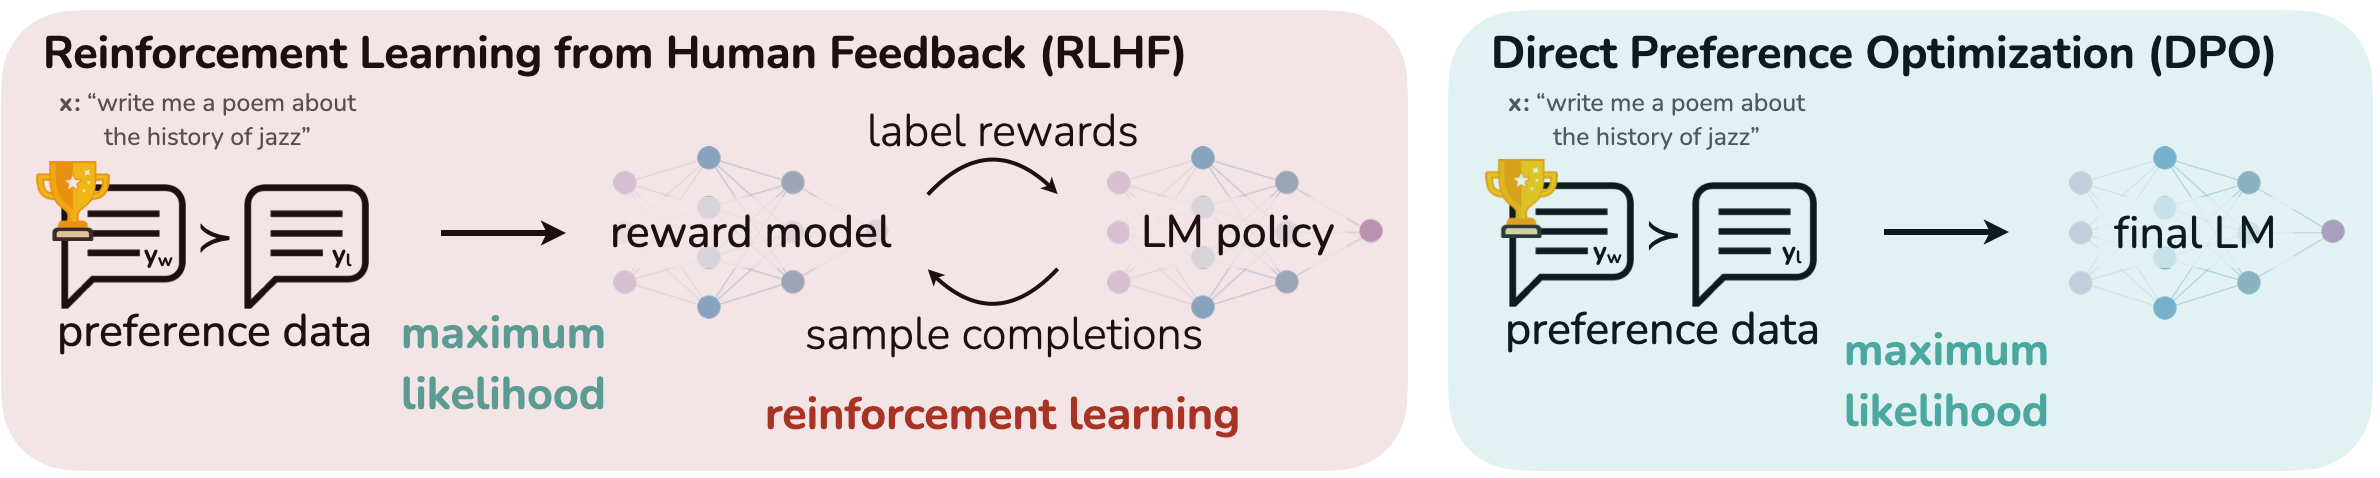
\includegraphics[width=15cm]{figure/teaser.png}
	\vspace{-0.2cm}
    \caption{\textbf{RLHF 和 DPO 的区别}}
    \label{fig:RHLFvsDPO}
	}
\end{figure}

通过将RLHF训练的3,4两步分别改用公式 \ref{DPOreward} 和 \ref{DPOpitheta},即得到了更为轻便高效的 DPO 训练流程。
图 \ref{fig:RHLFvsDPO} 展示了传统 RLHF 与 DPO 在训练上的过程对比。


\subsection{利用 LLM 构建偏好数据}

传统 RLHF/DPO 都需要大量人工的标注来训练奖励模型或直接在模型内进行偏好判断,
为了实现高效且可扩展的对齐过程,近年来利用 LLM 进行偏好数据集构建受到关注。  
一种常见的方法是让 LLM 生成多个对同一输入提示的响应,并利用 LLM 的预测来近似人类对这些响应的偏好,这种技术通常被称为 \textit{LLM-as-judge} \citep{bai2022training, yuan2024self}。  
然而,只有当 LLM 规模足够大且对齐良好时,该方法才能通过上下文学习有效地模拟人类偏好。  
另一种方法是使用外部奖励模型来替代人类偏好判断 \citep{jiang2023llm, snorkel2024pairrm},该方法可以更高效地进行偏好估计,但依赖于大量人类偏好数据来预训练奖励模型,并且在数据分布不匹配的情况下可能效果不佳。  
一些最新研究 \citep{rosset2024direct, snorkel2024pairrm, wu2024self, xiong2024iterative} 提出了结合迭代数据扩展与偏好学习的对齐方法,  
但它们通常依赖外部奖励模型或更强大的 LLM 进行偏好判断。  
相比之下,Dongyoung Kim 等发表的论文 \citep{Lee2024Rlaif,Yuan2024Self,Kim2025Spread}中提出了"Spread Preference Annotation"(SPA),它通过"模型自判断+自修正"的方式逐步扩展数据,
从而在仅有少量人工偏好标注的情况下也能获得良好的模型对齐效果。
论文的实验中仅利用训练中的 LLM 内在知识来进行新数据扩展和偏好学习。 
与常用的“外部奖励模型(RLAIF)”或用大模型做“LLM-as-judge”\citep{bai2022training, yuan2024self}不同,
论文强调让当前在训练的模型自身,根据它内部的输出概率(logits),直接判断新生成的响应哪个更好,即利用 DPO 的隐式奖励函数来对数据进行自标注。
因此,SPA 不需要额外的强大外部模型来判断,也不必依赖足够大型、已经高度对齐的人类偏好模型。
此外,论文还提出了一种"自我修正"或"降噪"的策略,来处理模型在自己打标签时可能产生的噪声(即错误的偏好判断)。
这一过程会识别出最有可能是错误标注的样本,并对它们的标注进行平滑或修正,从而减少被错误标签带偏的风险。

整个流程包括:
\begin{enumerate}
    \item 基于模型现阶段的参数去生成新的回答对,再对这对回答进行模型自判断;
    \item 然后将这些自标注的偏好数据与已有的小规模人工标注数据合并,进一步更新模型;
    \item 如此反复,形成迭代的"扩充-学习"循环。
\end{enumerate}
通过多次迭代,论文实验证明模型性能会显著提升。

\subsection{存在问题}

在前文已经讨论到,
传统方法通常需要大量精心策划的偏好数据集。
收集这样的数据集不仅代价昂贵且耗时,而且任何标签错误都可能在迭代对齐阶段传播 \citep{Casper2023Open},导致模型行为的次优甚至不安全。
这就提出了一个关键挑战:如何在保持对注释噪声的鲁棒性的同时,实现语言模型的偏好数据高效对齐?

从数据效率和鲁棒性的角度来看,现有的对齐方法通常面临两个主要问题:自我注释差距和噪声下缺乏平衡保证。
SPA中采用的自我注释 \citep{Lee2024Rlaif,Yuan2024Self,Kim2025Spread}的方法(即让LLM为新的提示-响应对生成标签,而不是依赖人工标签)
虽然确实降低了注释成本,但这些方法通常将策略更新和偏好注释视为不相关的过程。
因此,一旦生成了带噪声的合成偏好,如果 LLM 的自标签嵌入了系统性的偏差或错误,这些错误可能会破坏未来的训练 \citep{Chowdhury2024Provably},
而没有有效的补救措施。一些对抗训练方法 \citep{Cheng2023Adversarial,Wu2024Towards} 试图对抗偏好数据中的分布偏移,
但它们通常缺乏正式的平衡保证,并且在实际中可能导致不稳定的优化循环。
此外,这些对抗方法并未专门针对数据稀缺的对齐场景,因此在人工标签极其昂贵的情况下,其适用性有限。

\section{研究展望}

DPO 的训练范式具有很好的扩展性,而 SPA 的方法使得获取自动化的数据集成为可能,
在此基础上,探索更好的训练算法,在减少对于人工标注偏好数据需求的同时,也能较好保持对注释噪声的鲁棒性,是一个重要的研究方向。

一种可能的思路是采用基于对抗式训练的偏好优化方法,以提高大语言模型对人类偏好的对齐效率,特别是在数据高效性方面。
该思路需要考虑的问题主要有以下若干方面:首先,需要进一步优化对抗式训练过程中生成的对抗样本,
结合模型的自标注和对抗性重加权来生成数据,
进一步提升模型对真实世界应用中的异常情况和噪声数据的鲁棒性\citep{Esfahani2018Data};
此外,未来还可以通过探索更高级的对抗训练算法,提升模型在处理多样化噪声时的稳定性,
类似于DPO中处理潜在数据分布偏差的方式\citep{rafailov2023direct};
其次,对抗样本的支撑集也是需要考虑的一个因素,目前可能的思路是在已有数据的经验分布的临域内选取“最坏分布”
(对于临域的选择,可以考虑限定半径为 $\epsilon$ 的Wasserstein球),
以构造对模型最具有挑战性数据样本分布,在此基础上对模型进行不断的自增强训练,使得数据有效性和鲁棒性互相兼顾。
此过程类似于主从博弈中的对抗优化方法\citep{Bacsar1998Dynamic}。
此外,随着数据量的逐步增加,如何有效处理大规模的偏好数据并维持训练的高效性也是一个重要课题。
当前自标注的生成过程在大规模数据集上可能会面临计算和存储上的挑战。
因此,未来的研究可以考虑引入分布式训练和增量学习技术,
使得对抗式训练能够在更大规模的数据集上进行有效的扩展\citep{Villani2009Optimal}。

\newpage
\begingroup
    \linespreadsingle{}
    \printbibliography[title={参考文献}]
\endgroup